\section{Eredmények}
Az eredeti szimuláció választható mennyiségű test közötti gravitációs kölcsönhatás figyelembe vételével történt. Így a legegyszerűbb teszt maga a Naprendszer. A Föld és Nap adataival a "test" a következő fázisdiagrammhoz vezetetett:
\begin{center}
    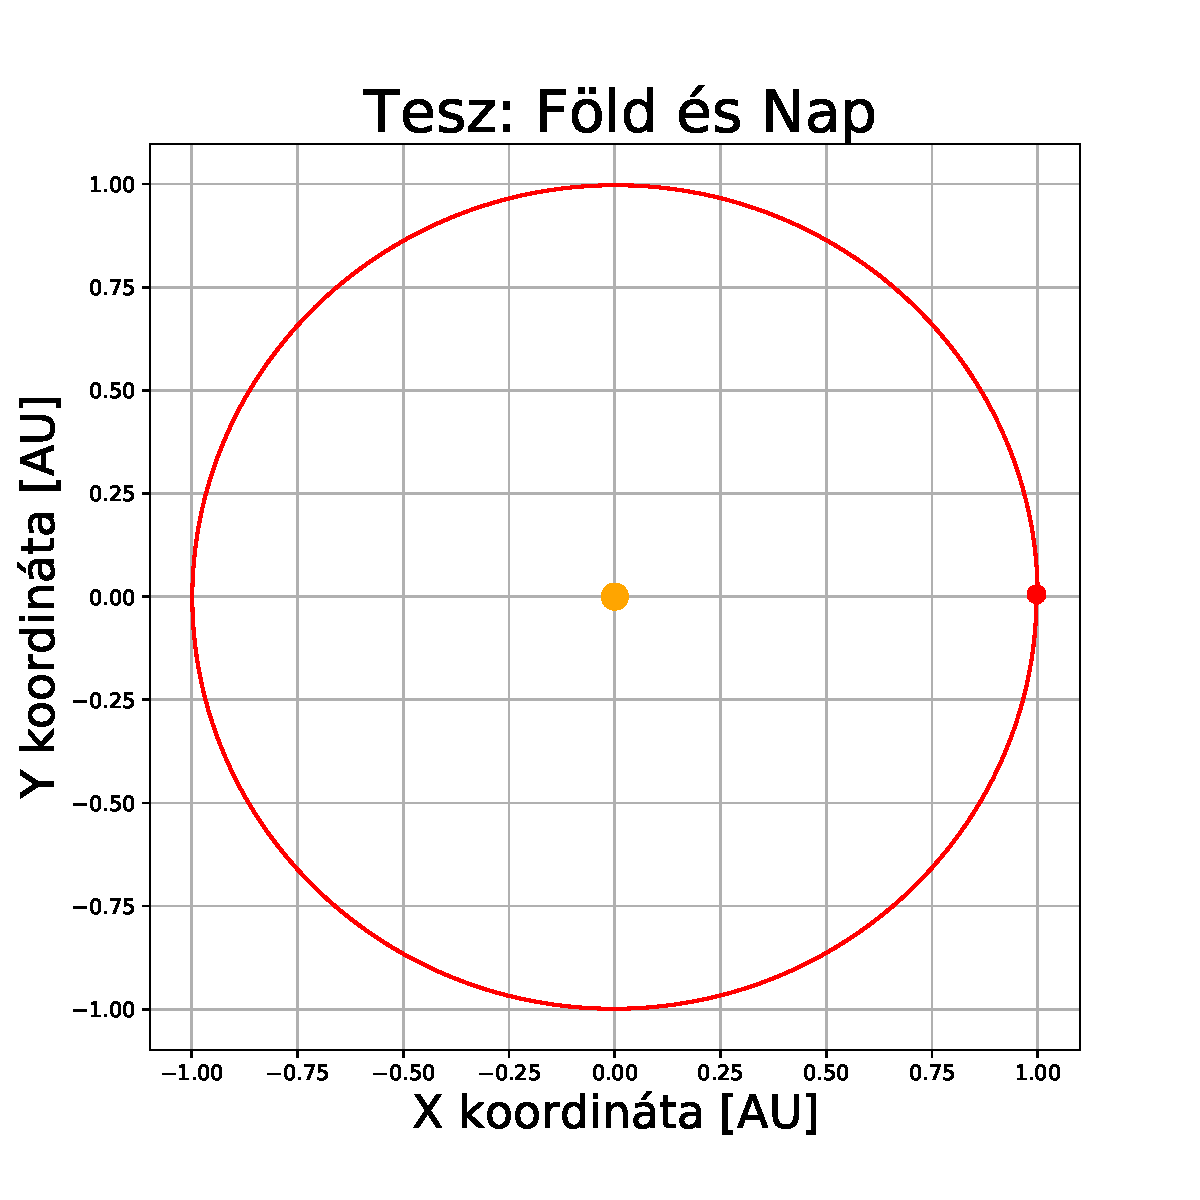
\includegraphics[width=0.7\textwidth]{pics/test1.pdf}
\end{center}
\captionof{figure}{Szimuláció a Földdel és Nappal.}
Láthatóan megfelelő pályát razol ki a fázisdiagram. A szimuláció egy év időtartamot ölel át. Ennek további vizsgálata viszont nem lényeges, hiszen a kinetikus és potenciál energia csak némileg változnak ezen időtartamon. Mivel közel ugyanoda érkezett vissza a bolygó, ezért látható (hosszabb időtartamú szimuláció esetén is) hogy a rendszer energiája megmarad.
Ezen egyszerú teszt megfelelő eredményt adott így egyből tovább is léptem a második tesztre: két csillag és egy bolygó. A "test2.txt" tartmalmazza ennek az adatait. A teszt sajnos kudarccal zárult:
\begin{center}
    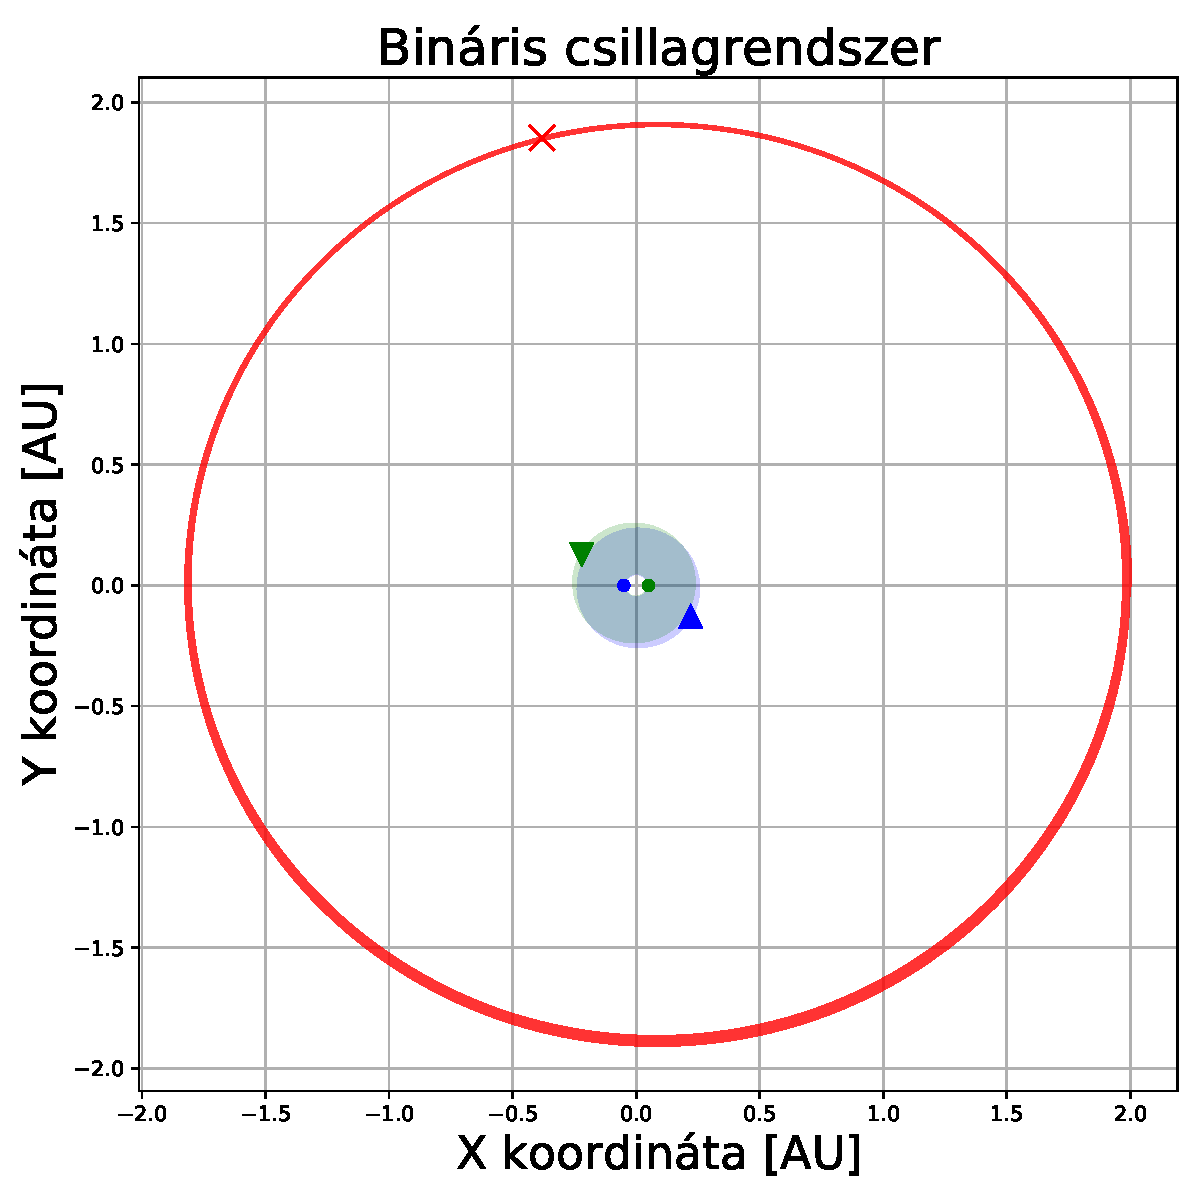
\includegraphics[width=0.7\textwidth]{pics/test2.pdf}
    \label{wrong_result}
\end{center}
\captionof{figure}{Egy bolygó két csillag körül. A jelöl pontok az utolsó állapotot jelölik, ami láthatóvá teszi a sikertelenségét.}
Ezen rendszernek szimulációja viszont teljesen sikertelen volt. Az utolsó állapotot egyértelműen rámutat, hogy a program valamely rész hibás, így pedig a mindig vonzó erő taszításba csap át. Ezen eredmény nem használható.
